\section{Systematic Uncertainties}
\label{sec:Systematics}

This section describes the range of systematic uncertainties
that are relevant for this analysis. To account for differences in the detector responses between simulation and data a 
set of corrections are applied either at object reconstruction level and at event level, 
the uncertainties on such corrections are considered as detector-related systematic 
uncertainties and are detailed in section~\ref{sec:sys:sys_det}. 
For samples which rely on MC simulation, theory-related
systematics, which include uncertainties on the cross-section and
uncertainties on the acceptance of analysis selections,  
are  described in section~\ref{sec:sys_theory}.
Further systematic uncertainties related to data-driven methods for backgrounds estimation
are described in section~\ref{sec:embsys} and~\ref{sec:qcdsys}.  

Each single systematic can contribute separately to the uncertainty on the
final event yield and on the shape of the $\mmc$
distribution which is used as discriminating variable in limit derivation. Shape systematics are
documented in appendix~\ref{appendix:shapeNPs}, they are found to be negligible for all the samples except
Embedding, for which significant deviation are found only in the b-veto category. 
Systematic uncertainties that do not effect the
mass shape distribution and have an impact on the event yield of less than 0.5\% (per sample) are 
neglected in the final limit calculations.
%hey infact do not have any significant effect on the final expected limits.


\subsection{Detector-related Systematics Uncertainties}
\label{sec:sys:sys_det}
Here systematic uncertainty related to object reconstruction and event 
corrections are addressed, those corrections are based on the measure of some relevant parameter, 
each of those parameters correspond to a "nuissance paremeter" in our probability model 
as described in Section~\ref{sec:ExclusionLimits}.
Each parameter is variated independently (one sigma up or down) according with its 
uncertainty and the impact on the analysis yield for each sample is evaluated.
In the following, detector related uncertainty are  described with some more details,
table~\ref{tab:ExpSys:btag} and~\ref{tab:ExpSys:bveto} briefly summarize the impact on the samples 
yield for the most significant systematic uncertainty considered. 


\paragraph{Luminosity}
The integrated luminosity of the 8 TeV data recorded at ATLAS during 2012 is measured to be $20.3 ~ fb^{-1}$ \cite{luminosity}, its uncertainty  is  2.8\%.

\paragraph{Pileup}
Simulated events are re-weighted to reproduce the average interactions per bunch crossing, $<\mu>$, seen in data. 
Those event weights has an uncertainty wich is propagated to each simulated sample.
%It has been seen
%that a proper description of the minimum bias vertex multiplicity is obtained if the $<\mu>$ 
%value in MC is first scaled by a factor of $1.11 \pm 0.03$ before re-weighting to match data. The uncertainty
%on this value is taken as a systematic uncertainty for the analysis.

\paragraph{Trigger Efficiency}
is corrected in simulation to match (as a mean value) the one in data, those correction weights 
are evaluated as a function of $\pt$ and $\eta$ of the leptons and have assciated uncertainties. 
Systematic uncertainties on both the single electron and electron-muon trigger efficiency are considered independently,  
those uncertainty range aproximately 1-2\%.

In the embedding sample, the trigger is emulated by applying weights to the event
topology in order to recover the right trigger efficiency, those weights are related to the one just described above
and have similar uncertainty. Trigger efficiency uncertainty for Embedding are considered uncorrelated with 
the one of other samples.

\paragraph{Electrons}
Two types of uncertainty on reconstructed electron objects are considered:
the first are related to electron identification and reconstruction efficiencies ("Electron ID"), 
the second type are related to electron energy scale and resolution corrections.
The energy scale uncertainties are split into a set of six different nuisance parameters, 
however, only few of them give a non negligible contribution. Two of them are found
to effect the shape of the \mmc distribution and are considered independently, those are the uncertainty
that arise from the $Z \rightarrow ee$ momentum measurement ("Electron Zee") 
and the one related to low momentum electrons ("Electron LOWPT"). 
All the other uncertainties related to energy scale and resolution are summed in quadrature ("Electron E").

\paragraph{Muons}
The uncertainty on muon identification efficiency depends on the charge and momentum of the muon.
Typically these uncertainties are of the order of a fraction of percent, and are referred as "Muon ID". 
The uncertainties on the muon energy scale and resolution are considerd independently for the inner detector 
and muon spectrometer measurements, then are added in quadrature to eastimate the final effect ("Muon E").

\paragraph{Taus}
Hadronic tau object are only used in the analysis as a veto. Uncertainties on both tau energy scale 
and identification efficiency have been investigated and are found to be negligible for this analysis.

\paragraph{Jets}
The systematic uncertainties on the Jet Energy Scale (JES) are split up into multiple sets of nuisance parameters, which
are related to different effects and components, for example the sensitivity to pileup or
to the flavour composition of the jet. The overall uncertainty on the JES ranges 
between 3\% and 7\%, depending on the $\pt$ and $\eta$ of the jet. To give an idea of the effect that these
uncertainty have on the analisis yield their sum in quadrature is reported in table~\ref{tab:ExpSys:btag} and~\ref{tab:ExpSys:bveto} as "JES", however
this is just a simplification for illustration purposes and in the limits extraction those uncertainties are considered uncorrelated.
Systematic uncertainty due to jet resolution ("Jet Resolution") are obtained by smearing the jet energy 
according to its uncertainty.
%The recommendation \cite{TWIKI_JETMET} to propagate each individual 
% source of uncertainty through the full analysis is followed. In this analysis the reduced set of fourteen uncertainties, know as 
% \verb=InsituJES2012_14NP=, have been considered: these include two uncertainties for eta intercalibration, four pile-up 
% uncertainties, a high-$\pt$ uncertainty and an uncertainty for MC non-closure. Of these, only the terms "JES Effective 1", 
% "JES Effective 2" and "JES Effective 3", the pileup uncertainty as a function of the number of primary vertices ("JES Pileup-NPV") and the uncertainty due to the jet area ("JES Pileup-Rho") have a significant effect on the event yields. Additionally, 
% the uncertainty related to the fraction of quark to gluon jets ("JES Flav. Comp") and on the different response to them ("JES Flav. Resp.") are considered. The additional uncertainty assigned to the b-jet energy scale, referred as "JES B", is also 
% significant to this analysis. Uncertainties related to theory and modelling ("JES EtaModelling") also contribute to this 
% analysis. Finally the effect of the jet energy resolution ("JES Resolution") is evaluated applying a smearing to the jets, the 
% resulting effect on the yield is symmetrised.

\paragraph{b-Tagging} is described in chapter~\ref{chap:detector}. Corrections are applied to simulation
to match b-tagging efficiency in data, uncertainties on the knowledge 
of the b-tagging efficiencies for the 70\% working point of the MV1 b-tagger are
considered. The effect of those uncertainties is evaluated independently in the cases of
 b-quark, c-quark and light or gluon initiated jets and referred respectively 
to as "B  Eff", "C Eff" and "L Eff". The tagging and mistagging efficiency uncertainties 
 are considered to be totally anti-correlated. 

\paragraph{Missing Transverse Energy}
The effect of the energy scale
uncertainties for all the physics objects is propagated to the \met calculation.
In addition uncertainty on the energy scale and resolution due to the remaining 
calorimeter energy deposit, the so called ``soft-terms'', are considered. All the
uncertainty on \met are independently propagated through the analysis and are
added in quadrature, this final term is referred as "MET" uncertainty.


%\paragraph{Summary} A summary of the effect of the experimental and theoretical systematic uncertainties on signal and background yields for the b-tag and b-veto channels are shown in Table~\ref{tab:ExpSys:btag} and Table~\ref{tab:ExpSys:bveto}, respectively. It should 
%be noted that the gluon fusion  signal sample suffers of poor statistics in the b-tag category. 
%Hence, some of the yield differences reported are statistically dominated for these samples.
%%	As a solution the mean value between all the sample mass point can be taken as measure of the single systematic, 
%However the gluon fusion production mode has a negligible contribution in b-tag category.
	
\begin{table}[tp]
  \centering
  \begin{tabular}{lccccc}
    \hline\hline
      	      		   \multicolumn{6}{c}{ b-tag category uncertainties (\%)}  \\
     \hline
      Source             & Signal bbH 	   & Signal ggH      & \Ztautau      &  Top 	& Other	 \\
    \hline
Electron ID  		 &2.3		   &2.6		     &	2.8          &1.8	&2.0	 \\
Electron E	  	 &0.7		   &1.2		     &0.5	     &0.5	&0.9	 \\
Electron LOWPT	  	 &0.4		   &0.0		     &0.4	     &0.1	&0.4	 \\ 
Electron Zee	  	 &0.3		   &0.6		     &0.4	     &0.6	&0.5	 \\
Muon ID 		 &0.3		   &0.3	   	     &0.3	     &0.3	&0.3	 \\
Muon E		  	 &0.5		   &0.8		     &0.1	     &0.1	&0.2	 \\
Trigger Single	Ele.  	 &0.7		   &0.5		     &0.5	     &0.8	&0.8	 \\
Trigger Dilepton  	 &1.0		   &1.2		     &1.4	     &0.6	&0.6	 \\
Embedding MFS	  	 &-		   &-		     &0.0	     &-		&-	 \\
Embedding Iso.	  	 &-		   &-		     &1.3	     &-		&-	 \\
JES		  	 &2.7		   &7.3		     &-		     &10.0	&7.0	 \\
JER		  	 &1.4		   &6.3		     &-		     &2.9	&3.0	 \\
B Eff		  	 &10.2		   &3.1		     &-		     &2.6	&5.0	 \\
C Eff		  	 &0.2		   &4.3		     &-		     &0.0	&1.2	 \\
L Eff		  	 &0.4		   &8.0		     &-		     &0.1	&1.2	 \\
Pileup			 &0.4		   &0.7		     &0.4	     &0.4	&0.9	 \\
MET 		  	 &0.7		   &0.5 	     &0.2	     &1.0	&1.2	 \\
%Acceptance		 &		   &		     &		     &		&	  \\
%Cross Section	  	 &-		   &-		     &5.0	     &5.5	&7.1	 \\
Luminosity	  	 &2.8 		   &2.8	 	     &2.8 	     &2.8 	&2.8 	 \\

    \hline
    \hline
  \end{tabular}
  \caption{Summary of the effect of the experimental systematic uncertainties on the yields of the different
	samples used  in the b-tag channel. Here "Other" refers to the sum of all the remaining samples: $\Wlnu$, 
	diboson, $\Zll$ and single top. The signal samples listed here are b-associated production and gluon 
	fusion with $m_{A}=120$ GeV and $\tan\beta=20$.} 

  \label{tab:ExpSys:btag}
\end{table}


\begin{table}
  \centering
  \begin{tabular}{lccccc}
    \hline\hline
      	      		   \multicolumn{6}{c}{ b-veto category uncertainties (\%)}  \\
     \hline
      Source             & Signal bbH & Signal ggH & \Ztautau &  Top 	& Other	 \\
    \hline
Electron ID  		 &2.4		   &2.3		     &2.9 (\bf{s})	     &1.4	&1.6	 \\
Electron E.	  	 &0.4		   &0.5		     &0.4	     &0.5	&0.9	 \\
Electron LOWPT	  	 &0.3		   &0.5		     &0.4 (\bf{s})	     &0.0	&1.2  \\ 
Electron Zee	  	 &0.4		   &0.4		     &0.4 (\bf{s})	     &0.1	&0.3	 \\
Muon ID 		 &0.3		   &0.3		     &0.3	     &0.3	&0.3	 \\
Muon E.		  	 &0.1		   &0.1		     &0.1	     &0.5	&0.5	 \\
Trigger Single	Ele.  	 &0.6		   &0.6		     &0.5	     &0.9	&0.9	 \\
Trigger Dilep.	  	 &1.0		   &1.0		     &1.3	     &0.2	&0.3	 \\
Embedding MFS	  	 &-		   &-		     &0.1 (\bf{s})   &-		&-	 \\
Embedding Iso.	  	 &-		   &-		     &0.0 (\bf{s})   &-		&-	 \\
JES		  	 &0.6		   &0.7		     &-		     &1.0	&1.2	 \\
JER		  	 &0.5		   &0.3		     &-		     &0.6	&0.3	 \\
B Eff		  	 &1.8		   &0.0		     &-		     &12.0	&0.8	 \\
C Eff	  		 &0.0		   &0.1		     &-		     &0.1	&0.0	 \\
L Eff	  		 &0.0		   &0.1		     &-		     &0.2 	&0.1	 \\
Pileup			 &0.5		   &0.8		     &0.4	     &0.3	&0.3	 \\
MET  		  	 &0.2		   &0.8 	     &0.1	     &0.2	&0.5	 \\
%Acceptance		 &		   &		     &		     &		&	  \\
%Cross Section	  	 &-		   &-		     &5.0	     &5.5	&5.9	 \\
Luminosity	  	 &2.8 		   &2.8	 	     &2.8 	     &2.8 	&2.8 	 \\

    \hline
    \hline
  \end{tabular}
  \caption{Summary of the effect of the experimental systematic uncertainties on the yields of the different
	samples used  in the b-veto channel. Here "Other" refers to the sum of all the remaining samples: 
	$\Wlnu$, diboson, $\Zll$ and single top. The signal samples listed here are b-associated production 
	and gluon fusion with $m_{A}=120$ GeV and $\tan\beta=20$. 
	 Shape uncertainty are noted with the symbol (\textbf{s}).} 
 \label{tab:ExpSys:bveto}
\end{table}



\subsection{Theoretical Uncertainties}
\label{sec:sys_theory}
%\subsection{Simulated Cross-Section Uncertainties}

Uncertainties on the cross-sections that have been used to normalise
simulation samples to data are reported in
Table~\ref{table:sys_xsec}. These
uncertainties include contributions due to parton distribution
functions (PDFs), the choice of the value of strong coupling constant,
and the renormalisation and factorisation scales.  Furthermore the
uncertainties on signal cross-section depends on $\tan\beta$, the
Higgs boson type ($A$/$h$/$H$) and mass.

The effect of systematic uncertainties due to various MC tuning
parameters, underlying event and
lepton kinematic description is considered.
Since the effect on the invariant mass distribution of the di-tau system from these systematic
uncertainties is negligible (as an example see
Figure~\ref{fig:theory_mass} ), only the variation in
acceptance is considered as systematic uncertainty.
The acceptance uncertainties for the ALPGEN Z MC, used for the normalisation of the embedded sample, 
are estimated at lepton preselection to be 4\% \cite{2010SMLLSupportNote}.
%\footnote{A bit old result, to be reviewed. Depends also on the
%embedding choice}
Since additional selections are applied directly to the embedded sample, 
no further acceptance uncertainties is considered. Acceptance systematics on
$t\bar{t}$ simulated events are estimated to be of 2\%. %\textcolor{red}{still to be added}.
%evaluated
%\footnote{also here is not totally clear yet} 
%by the difference between MC@NLO and POWHEG in
%the data-driven background estimate. 
%For other, single and dibosons
%production as well as single top production a 2\% uncertainty is
%assumed.
The acceptance uncertainties on diboson and single top production are assumed to be 2\%.
%\footnote{preliminary, this is following LEP-Had note, we
%  should cite some previous result here.}.
Uncertainties on signal acceptance have been estimated
by producing samples with varied MC generator parameters and evaluating, at
truth-level, the effect of analysis selections on leptons, taus and
jets. This truth-level study is implemented within the Rivet framework
\cite{RIVET}, where additionally b-tagging is performed by identifying b-quarks and applying
a weighting according to the estimated ATLAS b-tagging
efficiencies \cite{BtaggingScaleFactors}. The variation of the acceptance
with respect to the nominal MC tune has  been considered as
a source of systematic uncertainty. For signal a total acceptance 
uncertainty varies from 4\% to 30\% depending on $\mA$, production process 
and on the analysis category.

%The acceptance uncertainties of the two signal production modes are
%evaluated separately because of the use of different generators for each. For
%b-quark associated production, generated with SHERPA,
%the CKKW matching parameter $Q_{cut}$ has been varied from its default
%of $\sqrt{20 ~ GeV/E_{CMS}}$ to values of $\sqrt{15 ~ GeV/E_{CMS}}$
%and $\sqrt{30 ~ GeV/E_{CMS}}$. The factorisation scale was varied up
%and down by a factor of two and the renormalisation scale by a factor of
%10\%. Uncertainties due to the PDFs were determined by taking the RMS
%of the acceptance of the 52 error sets of the CT10 PDF set.  These
%effects are summarised in Table~\ref{table:sys_bba}. For a total
%uncertainty, all effects are summed in quadrature giving a total
%uncertainties that varies from 4\% to 30\% depending on $\mA$ and on the
%analysis category.  For gluon fusion production, generated with POWHEG
%and Pythia 8, the initial and final state
%radiation uncertainties were varied up and down, and the
%renormalisation and factorisation scales were varied simultaneously
%(the renormalisation scale by 10\% and the factorisation scale by factor 2\%).
%PDFs uncertainties were handled in the same way as for the $b$-quark
%associated production.  These variations are summarised in Table
%\ref{table:sys_gga}.  The uncertainties shown in Tables
%\ref{table:sys_bba} and \ref{table:sys_gga} are based on samples with
%$m_{A} = 120 \text{ GeV}$.  Results for the mass points 90, 200
%and 300 GeV are shown in Appendix \ref{appendix:additional} of this note.
 

\begin{figure}[tdp]
\begin{center}
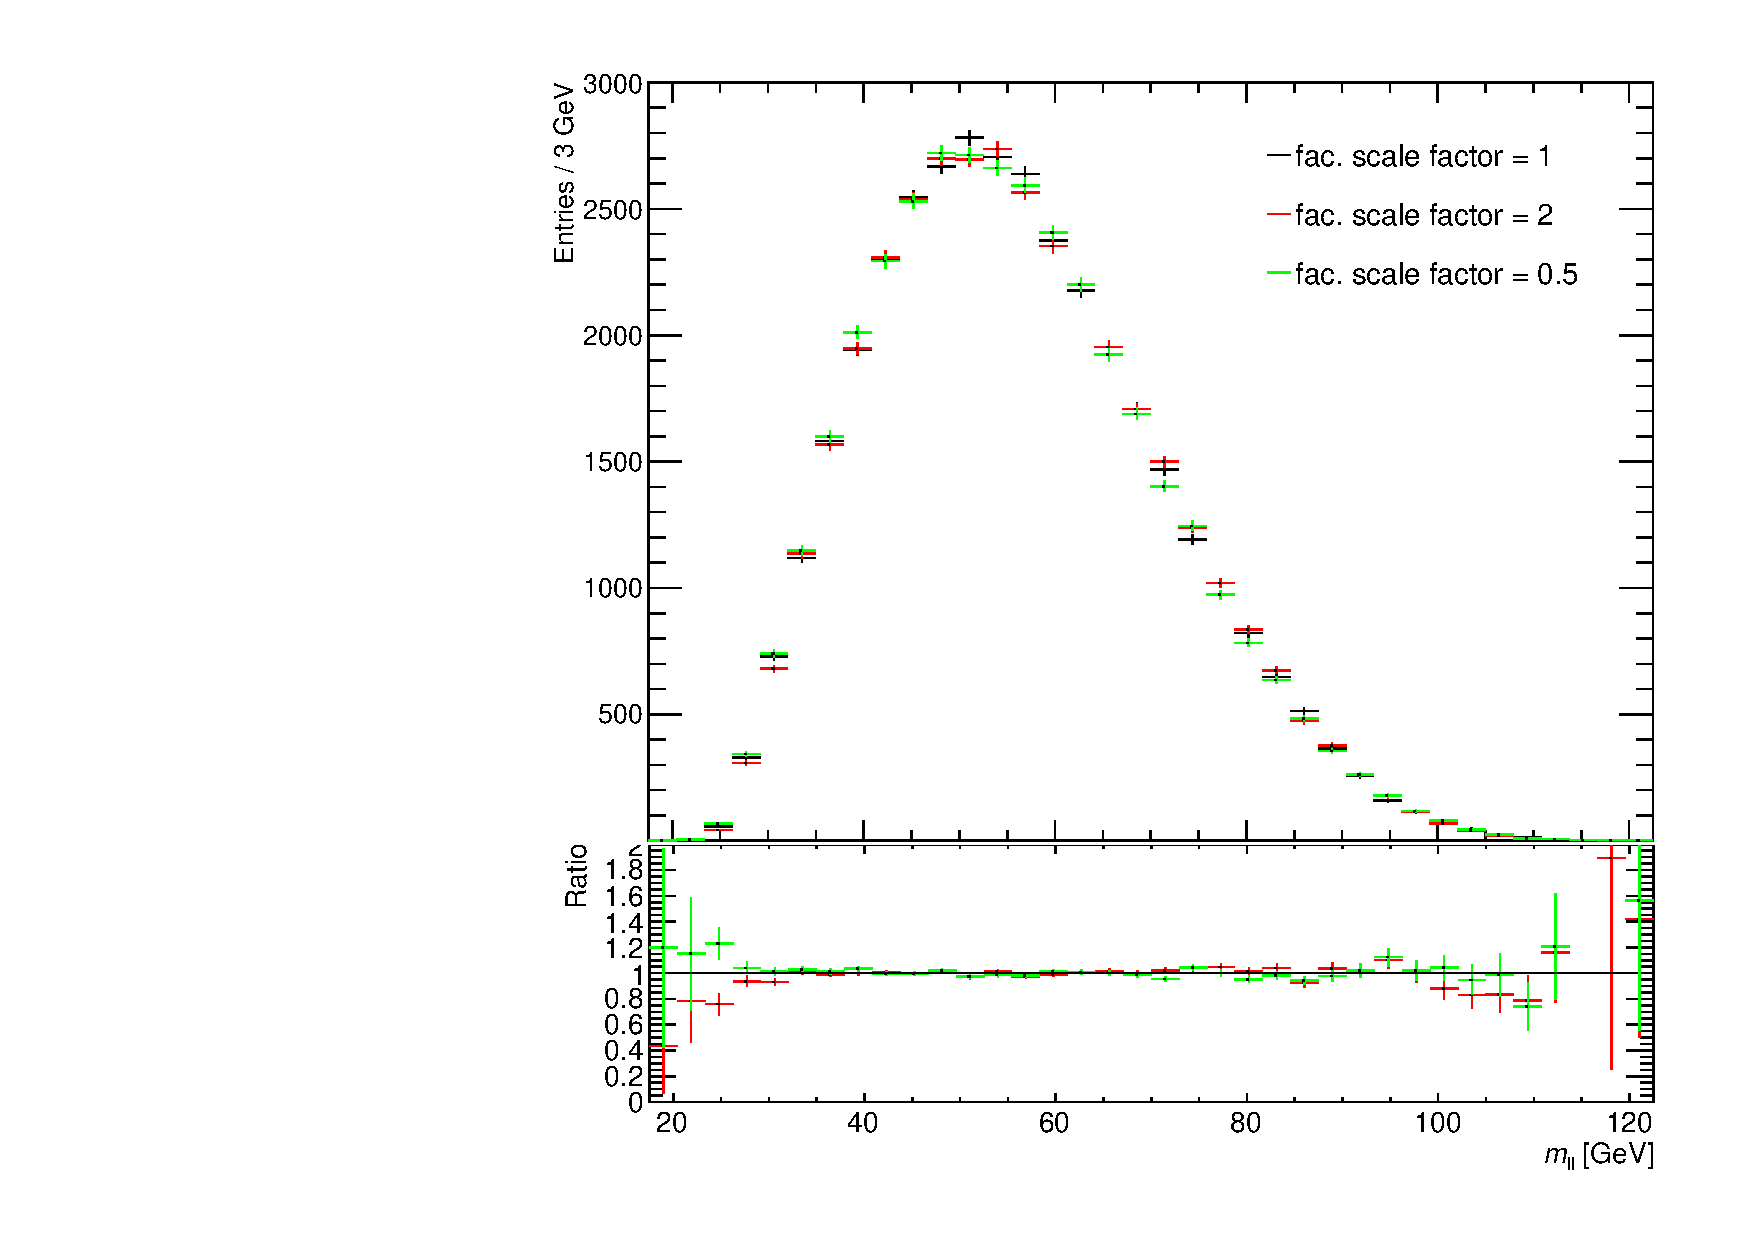
\includegraphics[width=8cm]{figure/facs_mll_bveto}
\end{center}
\caption{ Comparison of the visible mass of tau decay products after factorisation scale variation for the b-veto category on a gluon fusion signal sample.}
\label{fig:theory_mass}
\end{figure}


%\begin{table}[tdp]
%  \begin{center}
%   \label{table:sys_bba}
%   \begin{tabular}{lccccc}
%\hline \hline
% Event yields       & b-tag deviation [\%]  & b-veto deviation [\%] \\
%\hline
%CKKW down &    $ -3.1 \pm 0.9 $ &      $ 0.4 \pm 0.4 $ \\
%CKKW up &     $ -8.3 \pm 0.9 $ &      $ 2.9 \pm 0.4 $ \\
%Fac. scale down &    $ 15.5 \pm 1.0 $ &   $ -4.2 \pm 0.4 $ \\
%Fac. scale up &     $ -19.8 \pm 0.8 $ &    $ 5.6 \pm 0.4 $ \\
%Ren. scale down &      $ 0.4 \pm 0.9 $ &     $ -0.3 \pm 0.4 $ \\
%Ren. scale up &     $ 0.8 \pm 0.9 $ &      $ 0.5 \pm 0.4 $ \\
%PDF &     $\pm 0.1 $ 		& $\pm 0.2 $ \\
%\hline
%Total  (up) &     $ 13.5 \pm 1.6$ &                    $ 6.3 \pm 0.8$ \\
%Total  (down) &     $ -21.7 \pm 1.5$ &                    $ -4.2 \pm 0.6$ \\ 
%\hline \hline
%	\end{tabular}
%   \caption{Signal acceptances for several systematic deviations of the theory parameters contributing to the b-quark associated production of Higgs bosons. The different variations are added in quadrature to a total uncertainty on the signal acceptance in the b-tag and b-veto channels.}
%  \end{center}
%\end{table}
%
%
%\begin{table}[tdp]
%  \begin{center}
%   \label{table:sys_gga}
%    \begin{tabular}{lccccc}
 %   \hline \hline
% Event yields      &   b-tag deviation [\%] &   b-veto deviation [\%] \\
%\hline
%ISR up & $ 20.3 \pm 8.1 $ 		& $ -1.2 \pm 0.6 $ \\
%ISR down & $ 3.6 \pm 7.2 $ 		& $ 0.4 \pm 0.6 $ \\
%FSR up & $ 16.6 \pm 7.8 $ 		& $ -0.2 \pm 0.6 $ \\
%FSR down & $ -3.6 \pm 6.8 $	 	& $ -0.7 \pm 0.6 $ \\
%Ren./Fac. scales up & $ 9.4 \pm 7.5 $ 	& $ 0.0 \pm 0.6 $ \\
%Ren./Fac. scales down & $ 2.5 \pm 7.1 $ & $ -0.5 \pm 0.6$ \\
%PDF &     $\pm 0.0 $ &$\pm  0.1 $ \\
%\hline
%Total (up) &    $ 28.2 \pm 16.9 $ &     $ 0.4 \pm 0.6$ \\
%Total (down) &    $ -3.6 \pm 6.8 $ &     $ -1.5 \pm 1.2$ \\ 
%\hline \hline
%	\end{tabular}
%   \caption{Signal acceptances for several systematic deviations of the theory parameters contributing to the Higgs boson production through gluon fusion. The different variations are added in quadrature to a total uncertainty on the signal acceptance in the b-tag and b-veto channels.}
%  \end{center}
%\end{table}

\subsection{\Ztautau Embedding Systematics}\label{sec:embsys}

An important element of the embedding method is the subtraction of the 
calorimeter cells associated with the muons in the original \Zmumu event and their substitution with those from the simulated tau
decays. To make a conservative estimate of the systematic uncertainty on this procedure, 
the energy of the subtracted cells is scaled up or down by 30\%. The analysis is repeated with those modified 
samples and the relative uncertainty is referred as "EMB\_MFS", this uncertainty affects mainly the shape of the \mmc 
distribution, shown in figure~\ref{fig:EMBMFS}.

\begin{figure}[tp]
	\begin{center}
	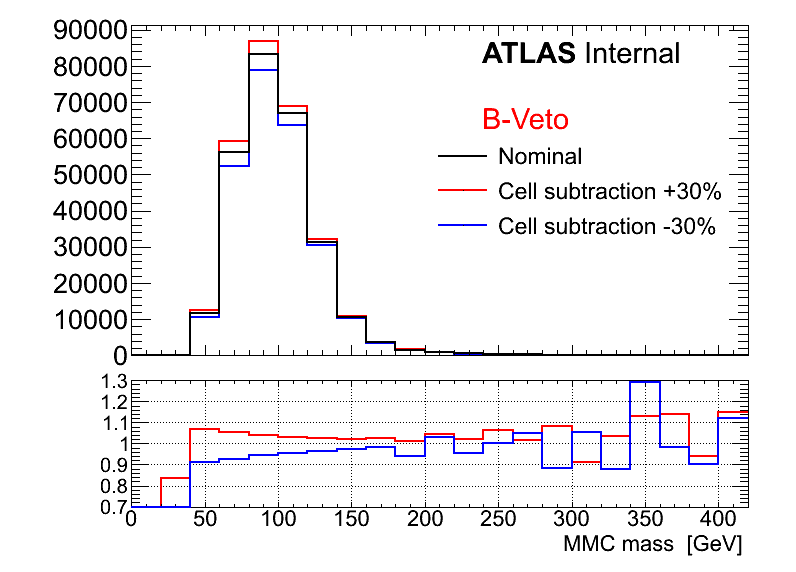
\includegraphics[width=0.49\textwidth]{figure/systematics/emb_sys_NoBtagFull_MFS.png}
	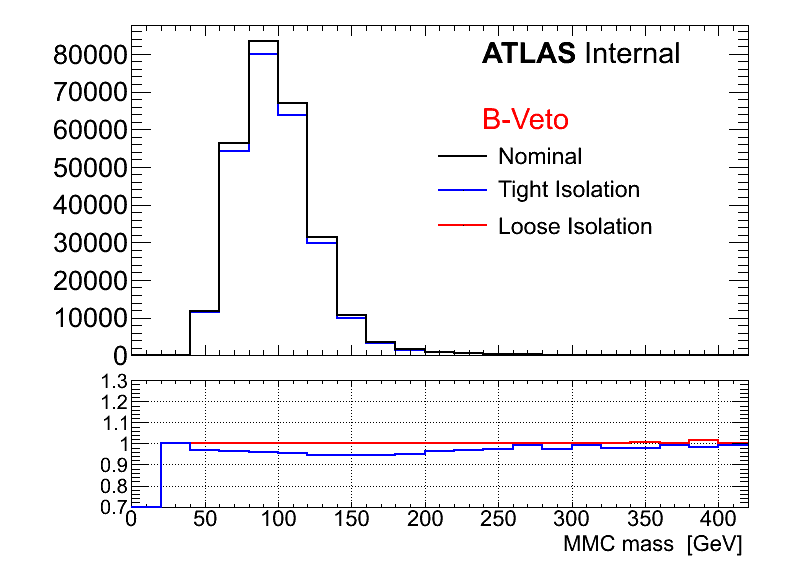
\includegraphics[width=0.49\textwidth]{figure/systematics/emb_sys_NoBtagFull_Iso.png}
	\end{center}
	\caption{Impact of EMB\_MFS (left) and EMB\_ISO (right) systematic uncertainties $\mmc$distribution for Embedding sample.
	Only the b-veto category report significant deviations.}
	\label{fig:EMBMFS}
\end{figure}

%\begin{figure}[htp]
%     \begin{center}
%
%        \subfigure[]{%
%            \label{fig:mvis}
%            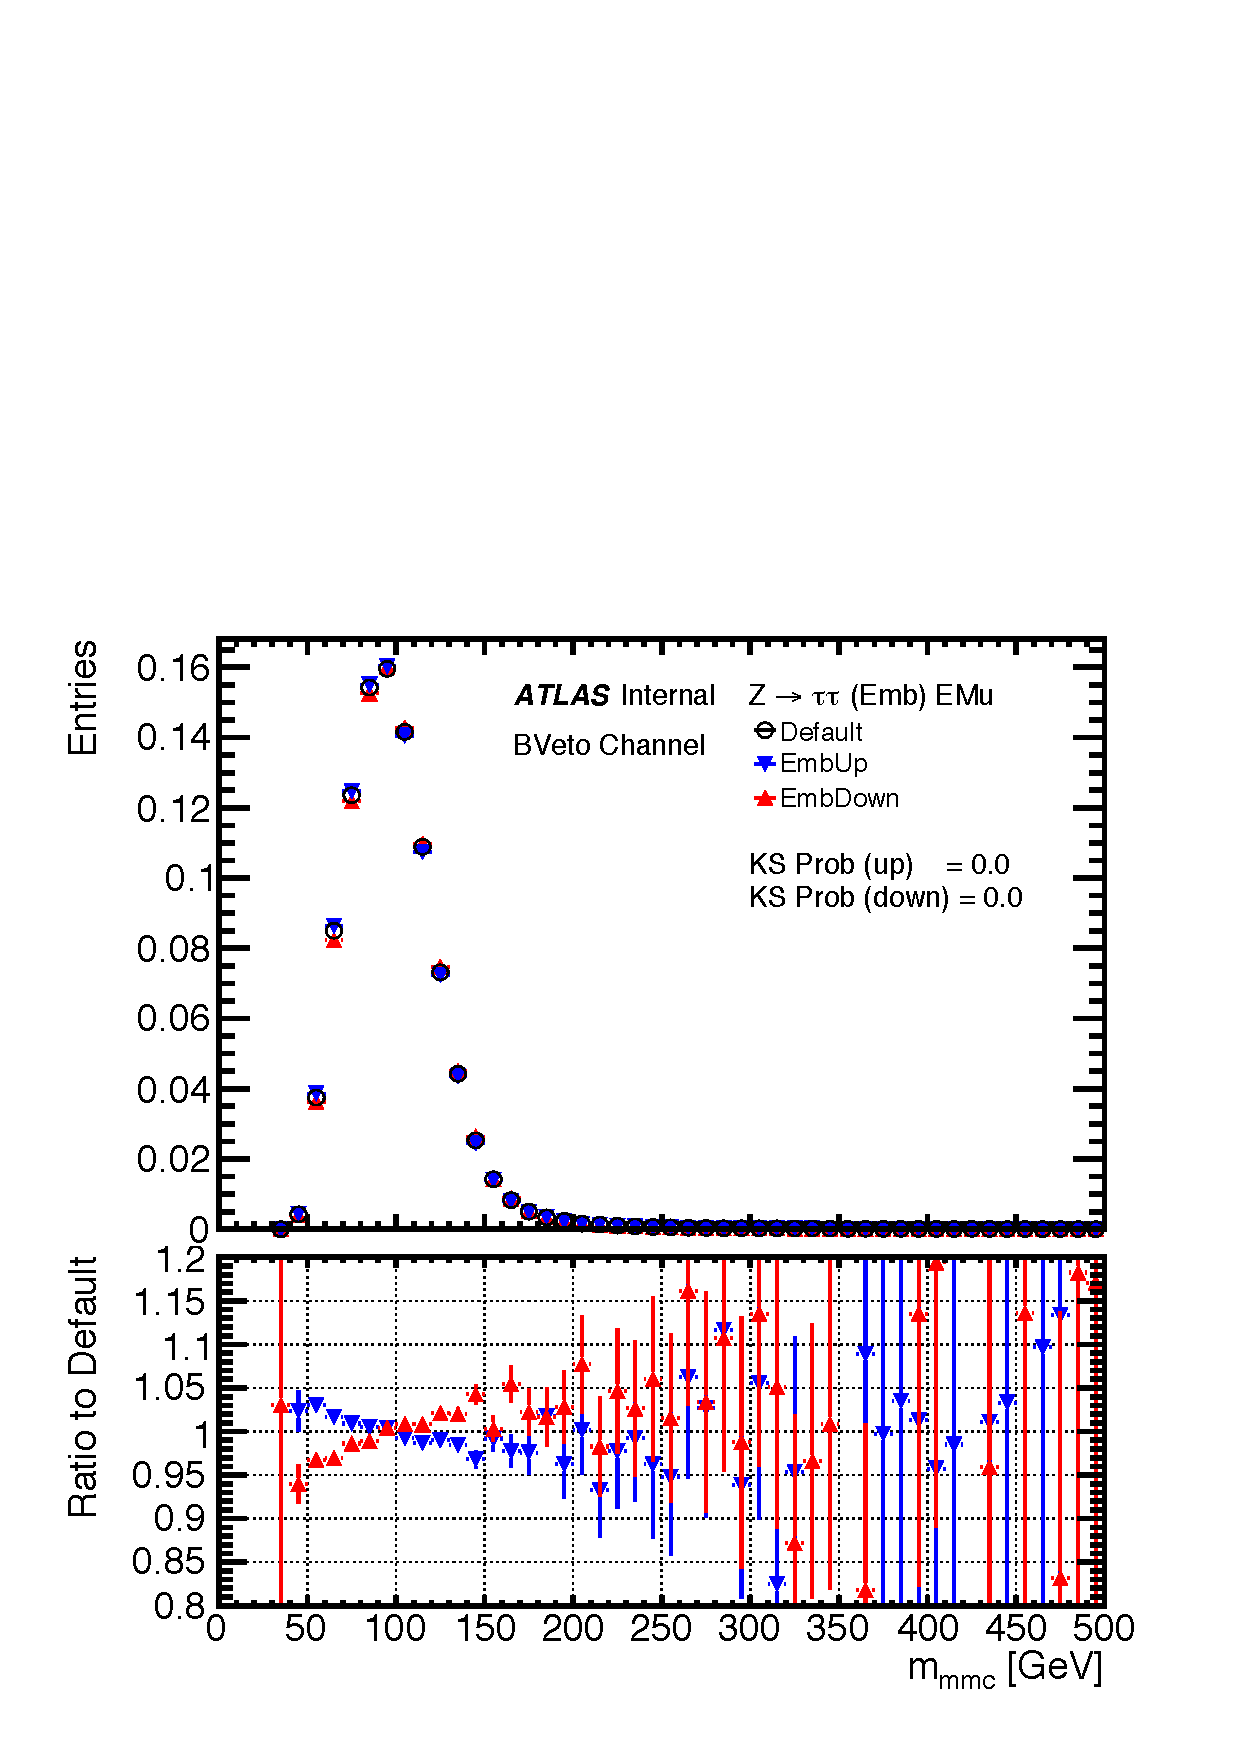
\includegraphics[width=0.45\textwidth]{figure/distributions/NP_Shape_EmbMFS_BVeto_mmc.pdf}
%	}
%	
%        \subfigure[]{%
%            \label{fig:mmc}
%            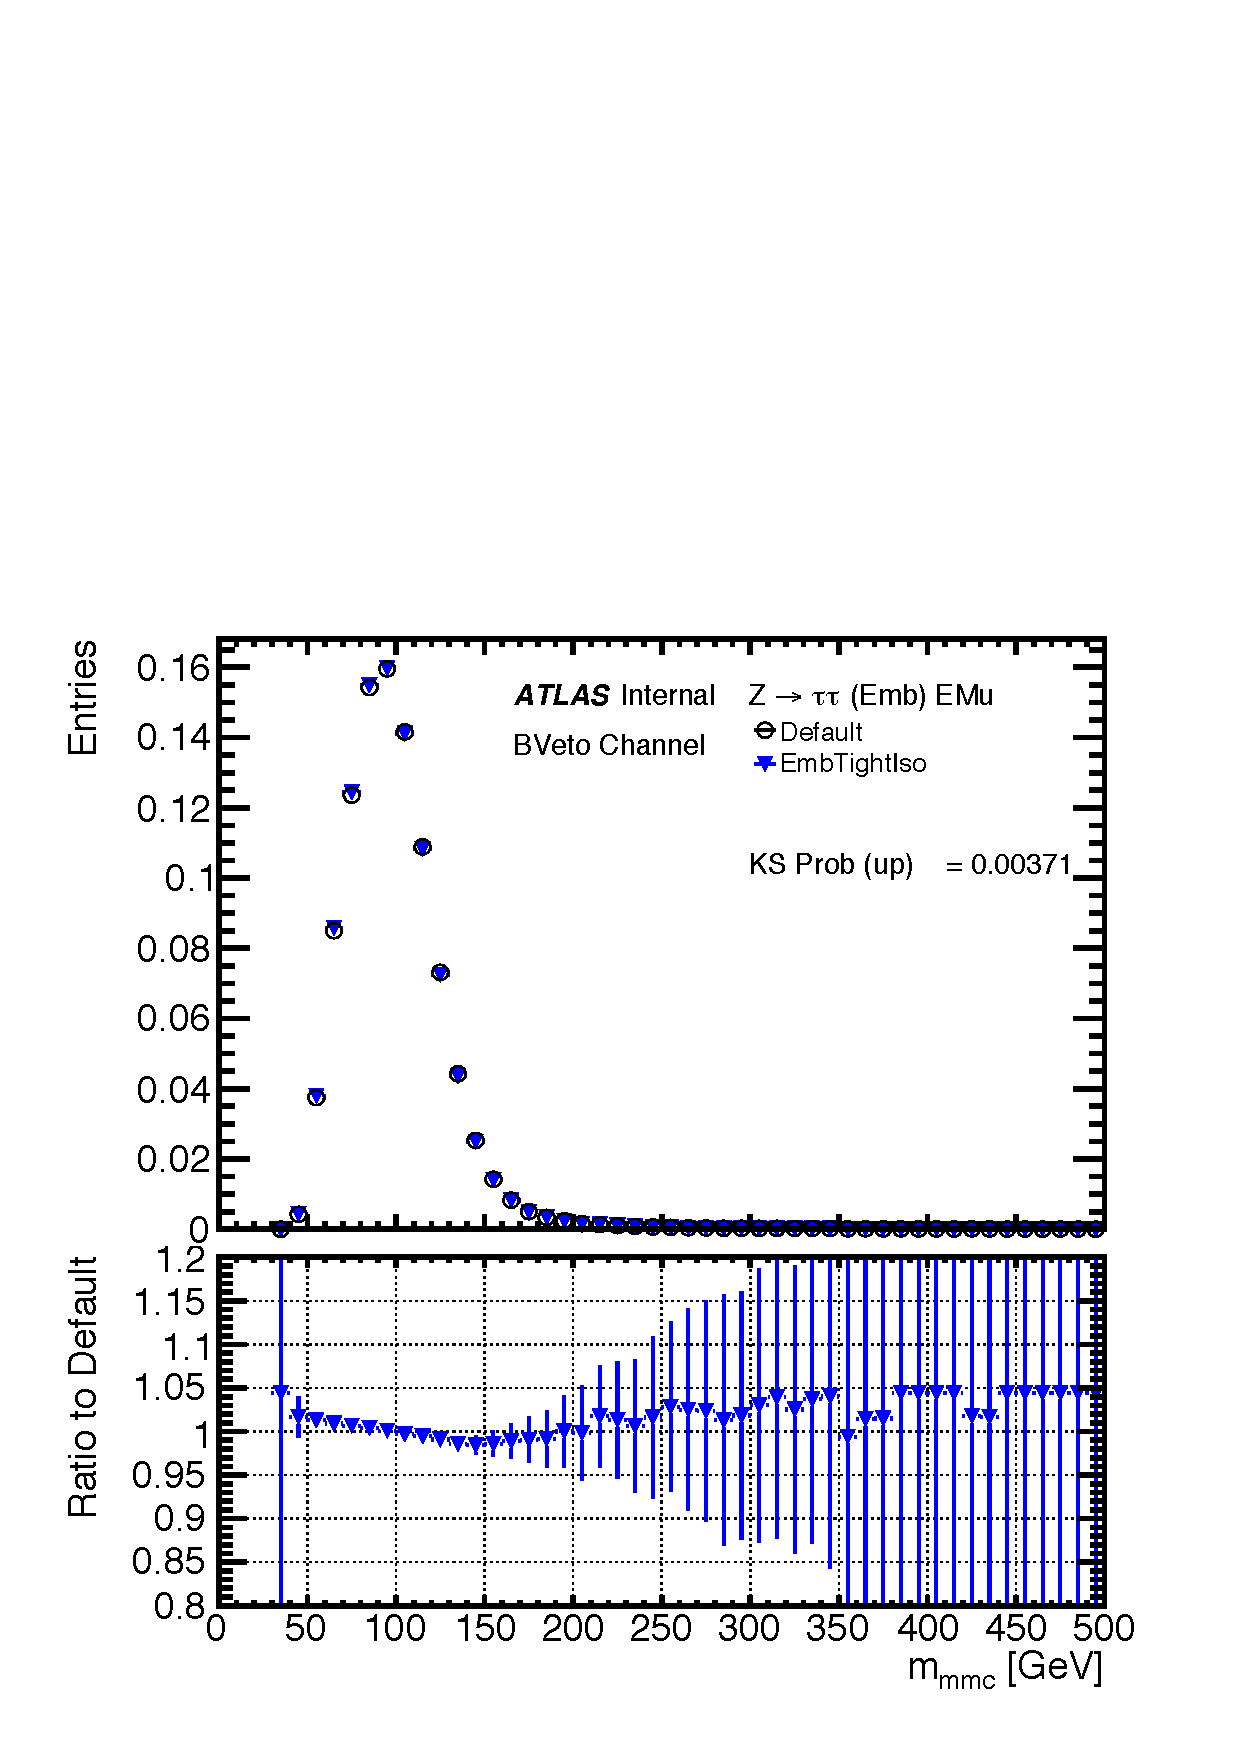
\includegraphics[width=0.45\textwidth]{figure/distributions/NP_Shape_EmbIso_BVeto_mmc.pdf}
%	}
%
%    \end{center}
%    \caption{Effect on the \mmc distribution of the embedding sample due to (a) the EMB\_MFS and (b) embedding isolation systematics. The plots are made after the full b-veto category selection.}
%   \label{fig:EmbeddingShapeNPs}
%\end{figure}

In the selection of the \Zmumu sample only a loose requirement on muon track isolation is required.
A different selection on the muon isolation may effect the selected sample by modifying the topology of the event, 
% since the requirement is indirectly acting also on the muon \PT, 
changing the non-\Zmumu contamination or the activity in the calorimeter. 
To estimate  the importance of these effects in our
embedding sample, the isolation selection on the muons in the original \Zmumu events is tightened,
%to $\ptcone 40/ \PT<0.06$ 
%and $\etcone 20/ \PT<0.04$, rather than the nominal selection of only $\ptcone 20/ \PT<0.2 $. 
a looser selection would have limited impact because of isolation requirements at trigger level.
The resulting uncertainty, referred to as "EMB\_ISO", affects both the yield and the \mmc shape of 
the embedding samples, as shown in figure~\ref{fig:EMBMFS}. 

Finally, because the normalisation of the embedding sample is determined by the use of the ALPGEN sample, 
the relative cross section and luminosity uncertainties are assigned. In addition
all the detector-related systematic uncertainties relevant to the decay products of the simulated tau 
decay are propagated to the embedding sample.
 
%\begin{figure}[tp]
%	\begin{center}
%	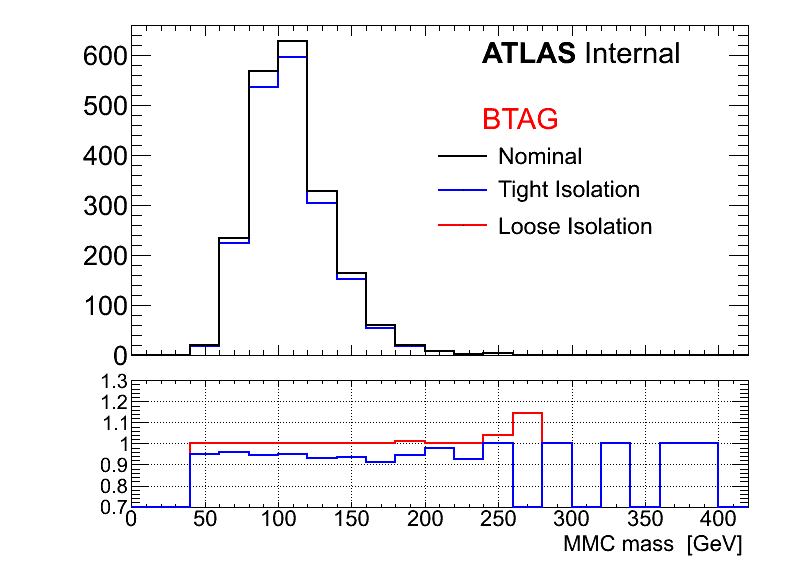
\includegraphics[width=0.49\textwidth]{figure/systematics/emb_sys_BtagFull_Iso.png}
%	\end{center}
%	\caption{Embedding Isolation systematic uncertainty impact $\mmc$.}
%	\label{fig:EMBISO}
%\end{figure}

\subsection{QCD Multi-Jet Systematics}\label{sec:qcdsys}

In this analysis the QCD multi-jet background is estimated via the ABCD method, as
described in Section~\ref{sec:qcd}. This technique relies strongly on
the assumption that the lepton isolation variables are independent from the
charge correlation between the two leptons. Systematic uncertainties
are assigned to take into account deviations from this assumption.
First the correlation between \rqcd and the lepton isolation selections is considered,
then the result is compared with an auxiliary method. 

Figure~\ref{fig:os_ss_ratio} shows the \rqcd factor, the ratio between the QCD 
yields in region C and D, as a function of the lepton isolation selections (red points).
%correlation is clearly visible. 
As described previously, the expectation from non-QCD backgrounds is subtracted from the data in regions C and D.
To estimate the uncertainty on the value of \rqcd  an additional transfer factor is defined as follows: $R_{QCD}^{iso}  = \hat{A} / \hat{B}$,
where  $\hat{A}$ and $\hat{B}$  are semi-isolated OS and SS regions defined with the lepton isolation larger than the standard requirement, 
but less than a sliding cut. Once more, the non-QCD contributions are subtracted from the data yields.
%$R_{QCD}^{iso}$ is an attempt to calculate a best estimate for the QCD transfer factor between isolated regions,
%which is in definitive the goal of the ABCD method. 
The regions $\hat{A}$ and $\hat{B}$ are chosen to be semi-isolated 
due to the high contamination of non-QCD background and possible signal in region A and B. 
Figure~\ref{fig:os_ss_ratio} shows $R_{QCD}^{iso}$ as a function of the lepton isolation selections (black points).
The difference between \rqcd and $R_{QCD}^{iso} $ in the vicinity of the standard cut value is then assigned as a systematic uncertainty on \rqcd. Using the point where the cuts on the lepton isolation are twice their standard values, a systematic uncertainty of 15\% is found.
The plot in Figure~\ref{fig:os_ss_ratio} is made at preselection level, similar plots using the full selection
for the two categories are in Appendix~\ref{appendix:qcd_additional}.

%for the definition of lepton isolations used in this analysis, the ratio is calculated in regions where the isolation requirements are reversed. Due to a high contamination of signal and non-QCD backgrounds, "semi-isolated" OS and SS regions are additionally defined, where the lepton isolation is larger than the standard requirement, but less than a sliding cut. These regions are labelled $\hat{A}$ and $\hat{B}$  for the semi-isolated OS and SS regions, respectively, and hence we can define $R_{QCD}^{iso}  = \hat{A} / \hat{B}$. The difference between \rqcd and $R_{QCD}^{iso} $ in the vicinity of our standard cut value is then assigned as a systematic uncertainty on \rqcd. Using the point where the cuts on the lepton isolation are twice their standard values, ie. the $x=100\%$ point on the graph, a systematic uncertainty of 15\% is found.

%An additional method considers calculating $\rqcd^{AB}$ as the ratio between the estimated QCD contributions in region A and B.
%These regions, however, suffers of large contribution of non-QCD background and possible signal contamination, 
%this method is then only used as a cross check. Table~\ref{table:MCsub} shows a comparison between \rqcd and  $\rqcd^{AB}$
%for the two category at an early stage of the cutflow where signal contamination is negligible, agreement is seen within statistical uncertainties.

An additional method, used as a crosscheck, considers calculating \rqcd as the ratio between the estimated QCD contributions in region A 
and B. Here the non-QCD contributions are once more subtracted from data. However the large contribution of this non-QCD background, 
along with lack of statistics and possible signal contamination, lead to this method being only used as a cross check. Table~\ref{table:MCsub} shows 
a comparison between \rqcd and $\rqcd^{AB}$ for the two categories at the preselection stage of the cutflow, where signal contamination is negligible. 
Agreement is seen between \rqcd values in the two regions, within statistical uncertainties. 

%\footnote{This effect is maybe due to the use of a \PT dependent isolation variable that effects the quark-gluon fraction.}.
%Expectation for non-QCD backgrounds are subtracted as usual. 
%This effect however doesn't tell anything on the uncertainty of our
%measure of \rqcd, we want to measure instead what is the discrepancy (for each
%choosen isolation cut value) between \rqcd and the same factor calculated 
%flipping isolation requirements, i.e. using the isolated regions A and B, we call this factor $R_{QCD}^{iso}$. 
%Due to the high contamination of non-QCD backgrounds and signal in these regions we then define:
%OS and SS isolated regions $\hat{A}$ and $\hat{B}$ in wich the leptons isolation
%should be greather than the standard value but less of predefined quantity on the x axis 
%of the graph (black curve). In definitive we have $R_{QCD}^{iso}  = \hat{A} / \hat{B}$.
%We then assign as a systematics uncertainty the difference between the two curves (red and black) in the vicinity of our
%standard cut value (we use the point where the cut value is doubled, 100\% in the graph because 
%of statistical fluctuation), our estimate of the systematics uncertainty on \rqcd is then 15\%.
%The plot in Figure~\ref{fig:os_ss_ratio} is made at preselection level, similar plots using the full selection
%for the two categories are in Appendix~\ref{appendix:qcd_additional}.

%An additional method used as a crosscheck relies on the definition of "real-$\rqcd$" as the pure ratio between region A and B (non-QCD background
%estimate is subtracted from data in each regions), this would be the exact factor 
%that allows you to extrapolate yield from region B to SR, however it suffer of contamination by non-QCD backgrounds
%and lack of statistics.
%Table~\ref{table:MCsub} shows comparison between \rqcd and real-\rqcd
%for the two category at an early stage of the cutflow where signal contamination is negligible.
%Discrepancies are within statistical uncertainty and underline that an assignment of a  15\%
%uncertainty to the \rqcd factor is conservative.


\begin{table} [tp]
	\begin{center}
	\begin{tabular}{l  c c c }
%%%%%%%%%%%%%%%%%%%%%%%%%%%%%%%%%%%%%%%%%%%%%%%%%%%%%%
\hline 
\hline
Selection  		&  \rqcd  			&  $\rqcd^{AB}$  		&  $R_{QCD}^{iso}$ \\ 
\hline
Preselection 		&   1.929 $\pm$     0.004	&	2.12 $\pm$ 0.17		&	2.22 $\pm$ 0.16	\\
B-veto			&  1.965   $\pm$   0.005    	& 2.10   $\pm$	0.16 		&	2.22 $\pm$ 0.16	\\
B-tag			&  1.78    $\pm$   0.02 	& 1.9   $\pm$	0.9 		&	2.0  $\pm$ 0.8	\\
\hline
\hline
%%%%%%%%%%%%%%%%%%%%%%%%%%%%%%%%%%%%%%%%%%%%%%%%%%%%%%
	\end{tabular}
	  \caption{Comparison between \rqcd, $\rqcd^{AB}$ and $R_{QCD}^{iso}$ for early stage in the cutflow, only b-tag and b-veto
	requirement are applied after preselections. Reported is statistical uncertainty only.}
	\label{table:MCsub}
	\end{center}
\end{table}


\begin{figure}[tp]
	\begin{center}
	\includegraphics[page=5,width=0.9\textwidth]{figure/QCD/qcd_plot.pdf}
	\end{center}
	\caption{OS/SS ratio as a function of lepton isolation variable selections. The selections are varied as a percentage relative to
	the standard lepton isolation cut values (0~in the plot). 
	%As an example the point at 100\% in the plot corresponds
	%to $\rqcd$ evaluated by increasing the isolation requirement by 100\% respect to the standard cut value.
	The red points show the anti-isolated scale factor $\rqcd$, i.e. the ratio between regions C and D.
	 The black points show the isolated scale factor, which is defined as the ratio between region $\hat{A}$ and $\hat{B}$, 
	 where the leptons have isolation values larger than the nominal value but smaller
	 than the sliding cut on X axis.
%	 taking the same example point at 100\%, than the double of the standard cut value.
	 }
	\label{fig:os_ss_ratio}
\end{figure}

The difference in \mmc shape observed between the OS and SS anti-isolated regions (C and D) is shown in Figure~\ref{fig:qcd_shape_unc}.
This effect is within the  uncertainty on \rqcd of the ABCD method, hence no correction factor is applied to the mass shape. We assume, however, that there could be the same 
shape difference in the isolated regions, a shape uncertainty is then assigned to region B to take into account this  deviation. Further 
shape uncertainties due to non-QCD background subtraction are found to be negligible. The uncertainty due to the use of an isolation 
requirement at trigger level is discussed in Appendix~\ref{appendix:qcd} and is found to be negligible.


\begin{figure}[tp]
	\begin{center}
	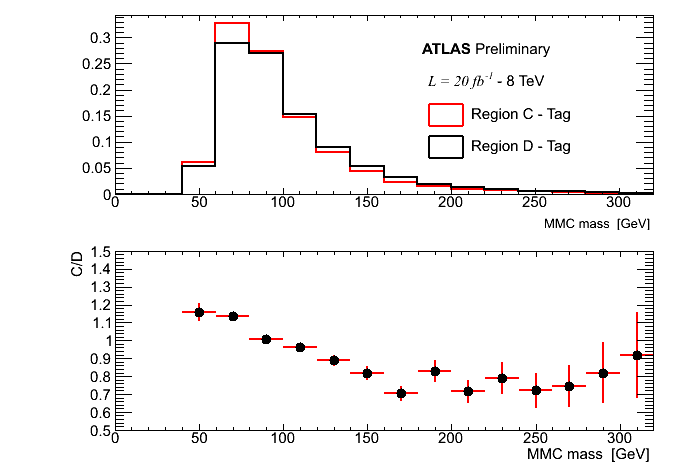
\includegraphics[width=0.65\textwidth]{figure/QCD/shape_tag.png}
	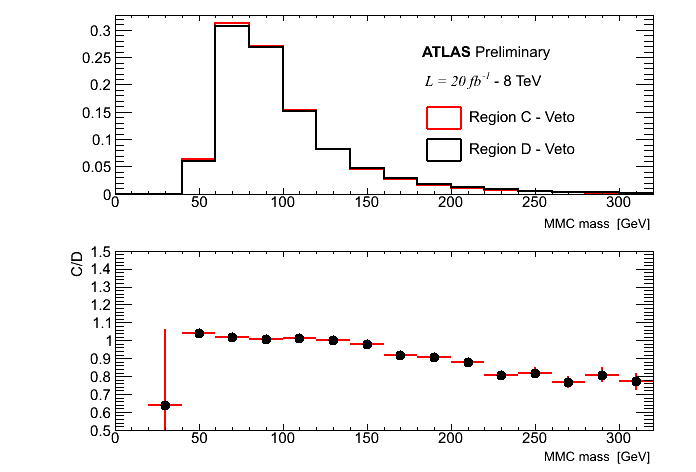
\includegraphics[width=0.65\textwidth]{figure/QCD/shape_veto.png}
	\end{center}
	\caption{Shape differences for the b-tag and b-veto categories between the ABCD regions C and D.}
	\label{fig:qcd_shape_unc}
\end{figure}






\begin{table} [t]
\centering
\begin{tabular}{c c c }
\hline
\hline
Generator & Process & Uncertainty \\ [0.5ex]
\hline
ALPGEN & $Z \rightarrow \tau\tau / ee /\mu\mu$ & $\pm 5\%$ \\
POWHEG & \ttbar					& $\pm 5.5\%$\\
ALPGEN & $W  \rightarrow \tau\nu / e\nu /\mu\nu$&  $\pm  5\%$ \\
AcerMC & single top & $\pm 13 \%$ \\
HERWIG & dibosons & $\pm 6 \%$ \\
SHERPA & $bbA$/$h$/$H$  ($m_{A} \ge 120$~GeV)     & $-(<20)$\%,  $+(<9)$ \%\\
SHERPA & $bbA$/$h$/$H$  ($m_{A} =   110$~GeV)     & $-(<25)$\%,  $+(<9)$ \%\\
SHERPA & $bbA$/$h$/$H$  ($m_{A} =   100$~GeV)     & $-(<28)$\%,  $+(<9)$ \%\\
SHERPA & $bbA$/$h$/$H$  ($m_{A} =    90$~GeV)     & $-(<30)$\%,  $+(<9)$ \%\\
POWHEG & $ggA$/$h$/$H$  ($m_{A} \le 300$~GeV)     & $<$ 15\%\\  [0.5ex]
\hline \hline 
\end{tabular}
\caption{Cross-section uncertainties for background and signal samples.The reported signal samples are all for $\tan\beta = 20$.}
\label{table:sys_xsec}
\end{table}


